% This must be in the first 5 lines to tell arXiv to use pdfLaTeX, which is strongly recommended.
\pdfoutput=1
% In particular, the hyperref package requires pdfLaTeX in order to break URLs across lines.

\documentclass[11pt, round]{article}

% Remove the "review" option to generate the final version.
\usepackage{acl}
\usepackage{gb4e}
\noautomath
% Standard package includes
\usepackage{times}
\usepackage{latexsym}

\usepackage{graphicx}
\usepackage{caption}
\usepackage{subfig}
\graphicspath{{./img/}}

% For proper rendering and hyphenation of words containing Latin characters (including in bib files)
\usepackage[T1]{fontenc}
% For Vietnamese characters
% \usepackage[T5]{fontenc}
% See https://www.latex-project.org/help/documentation/encguide.pdf for other character sets

% This assumes your files are encoded as UTF8
\usepackage[utf8]{inputenc}

% This is not strictly necessary, and may be commented out,
% but it will improve the layout of the manuscript,
% and will typically save some space.
\usepackage{microtype}

\usepackage{natbib}
\bibliographystyle{plainnat}

\title{Do LSTMs Understand the Licensing of Negative Polarity Items?}

\author{Theo Sandstrom \\
  \texttt{theo.sandstrom@yale.edu} \\
  Trey Skidmore \\
  \texttt{trey.skidmore@yale.edu} \\
  Prastik Mohanraj \\
  \texttt{prastik.mohanraj@yale.edu}}

\begin{document}
\maketitle

\begin{abstract}
While LSTMs have proven themselves as powerful tools for language modeling tasks, the extent to which their generalizations are based on underlying syntactic structure remains an open area of inquiry. We focus our investigation on the relationship between negative polarity items (NPIs) and their licensors in English. We probe the model's representation of this relationship by computing the network's surprisal upon encountering NPIs in licensed and unlicensed environments. While we do observe that the inclusion of a licensor causes a significant reduction in model surprisal, we do not observe any change in surprisal depending on whether or not the licensor c-commands the negative polarity item. 
\end{abstract}

\section{Introduction}

The development of Recurrent Neural Networks (RNN) has been a recent hallmark of advancements in Natural Language Processing (NLP). The inherent ability for RNNs to learn and internalize a number of linguistic capabilities is evidenced by a large corpus of research in the utilization of RNNs for NLP tasks such as machine translation, language modeling, and syntactic parsing \cite{wilcox-etal-2018-rnn,gulordava2018colorless,jozefowicz2016exploring}. 

However, it is still largely unknown how such networks represent linguistic information internally. Historically, the majority of research on these networks has focused simply on evaluating and optimizing performance on applied NLP tasks. However, there has been a recent increase in literature probing inside of these black box models and evaluating the extent to which their success is based on surface level heuristics rather than genuinely extracting and interpreting structural properties of language, either syntactic or semantic. \cite{lakretz2019emergence}.

One subset of RNNs, namely Long Short-Term Memory RNNs (LSTMs), has grown in utility in said extraction of structural properties of language. Wilcox et al. \shortcite{wilcox-etal-2018-rnn} researched the ability of LSTM models to learn the syntactic filler-gap dependency, the relationship between a filler word (in English, a wh- complementizer like \textit{what} or \textit{when}) and a gap word (in English, an empty syntactic position uniquely licensed by a filler word). Lakretz et al. \shortcite{lakretz2019emergence} similarly explored the ability of LSTM models to identify numerical agreement between verbs and their arguments. 

There is, though, little research investigating the feature of licensing of negative polarity items in language. Negative polarity items are a class of words that are only permitted to appear in certain "negative" contexts. For example, in English, negative polarity items include words like \textit{ever}, \textit{any}, and \textit{even}.
\begin{enumerate}
    \item He never gave up.
    \item *He \textit{ever} gave up.
    \item Nobody ever gave up.
\end{enumerate}
Here, the word \textit{ever} is not permitted to occur in a sentence except when licensed by a word such as \textit{nobody} that provides the surrounding "negative" context. Notably, the relationship between the licensor and the negative polarity item is based on the hierarchical structure of a sentence, wherein the licensor must c-command the negative polarity item (i.e. the negative polarity item must be a sister of the licensor or a direct descendant of a sister node of the licensor).

If a language model after being trained on a generic linguistic data set is able to predict the distribution of negative polarity items and the contexts in which they are licensed with significant accuracy, this would be evidence that the model is able to learn this feature of syntax, in particular that it is able to detect a relationship between a licensor and a negative polarity item.

\section{Methods}

\subsection{Language Model}

For our investigation, we trained a LSTM model on the WikiText-2 dataset \cite{merity2016pointer}, which consists of over 2 million tokens from 600 Wikipedia articles, with a vocabulary size of 33,279. Our LSTM has an embedding layer, assigning 200-dimensional embeddings to each word in the vocabulary, and two recurrent layers, each with 650 hidden units. During training, we use dropout regularization as described in Srivastava et. al. \shortcite{srivastava2014dropout}, with a dropout rate set at 0.2. Optimization was performed using gradient descent, with a base learning rate of 0.2, which decreased exponentially whenever performance on the development set regressed.

The model can be found in the project's GitHub repository (\url{https://github.com/tsandstr/ling380-final-project}).

\subsection{Surprisal}

We assess the ability of an LSTM to predict the distribution of negative polarity items by using the surprisal metric, as applied in Wilcox et. al. \shortcite{wilcox-etal-2018-rnn}. The metric is defined to be the log inverse probability:
\[ S(x_i) = -\log_2 P(x_i \, | \, h_{i-1}), \]
where $x_i$ is the current word, $h_{i-1}$ is the LSTM's hidden state before $x$ and the probability is given by the softmax activation. The surprisal is measured in bits because we take a base two logarithm.

A high surprisal metric means that, in the given context, a word was predicted with \textit{low} probability, and was therefore unexpected by the model. Basically, given a hidden state of the model at a current time step, the surprisal metric is a way to measure the whether the next word makes \textit{sense}. A direct correlation has been shown between language model surprisal metrics and  human sentence processing difficulty \cite{hale2001probabilistic,levy2008expectation,smith2013effect}. 

\subsection{Experimental Design}

\section{Representation of Negative Polarity Items}

Negative polarity items have a variety of linguistic properties which we would like to probe. On the most basic level, they are only allowed to occur in negative contexts. More specifically, in order for an NPI to be licit, it must be c-commanded by its licensor. Another property is that NPIs are immune to intervening material separating the NPI from its licensor. And finally, one negative context can license multiple negative polarity items. In this section we demonstrate that LSTMs have learned these four properties negative polarity items.

Our general approach to studying these properties of the dependency between NPI and licensor is as follows. We construct a number of test items containing negative polarity items, including variation in whichever independent variable we are curious about (e.g. whether or not the licensor c-commands the NPI). For each item, we construct two variants: one with a licensor, and one without a licensor. We define the licensing interaction to be the difference in surprisals between these two variants:
\[ \textrm{interaction} = S_{\textrm{no license}} - S_{\textrm{license}}. \]
A large licensing interaction suggests that, in a given test item, the presence of a licensor does dampen the model's surprisal at encountering an NPI, while a small licensing interactoin suggests that, in a given test item, the licensor does not dampen the surprisal.

In computing the licensing interaction, we measure surprisal in two different ways. First of all, we can measure the instantaneous surprisal of the model upon encountering an NPI. Secondly, we measure cumulative surprisal from the NPI to the end of its clause. We measure instantaneous surprisal because we expect the grammaticality of an NPI to have some local effect on the model's predictions. We measure cumulative surprisal because we expect the grammaticality of an NPI to have longer-reaching effects on the model's predictions for the whole sentence.

\subsection{Licensing of Negative Polarity Items}

As discussed in the introduction, negative polarity items are only grammatically allowable in negative contexts. The following examples demonstrate this fact because only the sentences with negative contexts (a,c) are grammatically permissible:
\begin{exe}
\ex\label{ex:license-1}
\begin{xlist}
\ex Bill is not here yet.
\ex[*]{Bill is here yet.}
\end{xlist}
\ex\label{ex:license-2}
\begin{xlist}
\ex They hired somebody without any talent.
\ex[*]{They hired somebody with any talent.}
\end{xlist}
\end{exe}
In this subsection, we confirm the hypothesis that surprisal metrics for NPIs are reduced in the presence of an appropriate licensor. As described above, we created 20 test items containing negative polarity items, and for each item, we constructed one variant with a licensor, and one without a licensor, as exemplified in Examples \ref{ex:license-1} and \ref{ex:license-2}.

Plotted in Figure \ref{fig:surprisal-basic-licensing} are graphs of surprisal on two generic examples; negative polarity items are assigned lower surprisal values by the model when they are found in grammatically licit environments. 

\begin{figure}
    \centering
    \subfloat[Grammatical]{{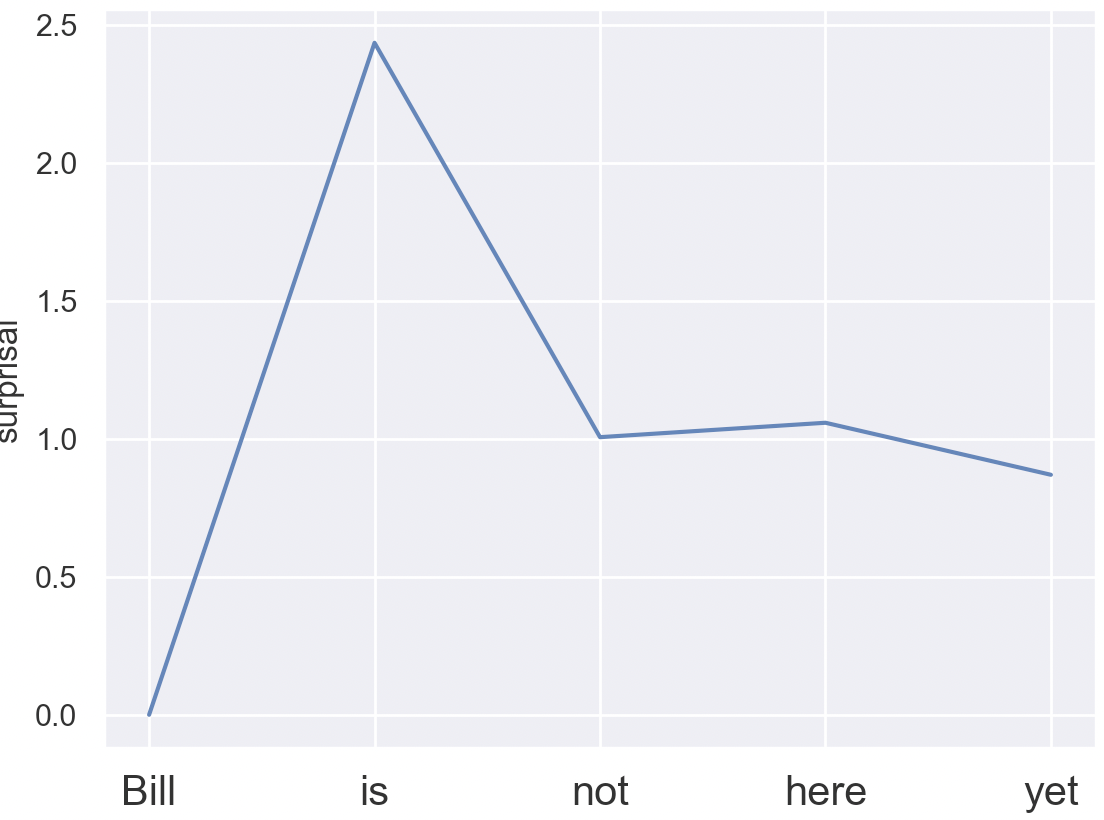
\includegraphics[width=.42\linewidth]{good1} }}
    \subfloat[Ungrammatical]{{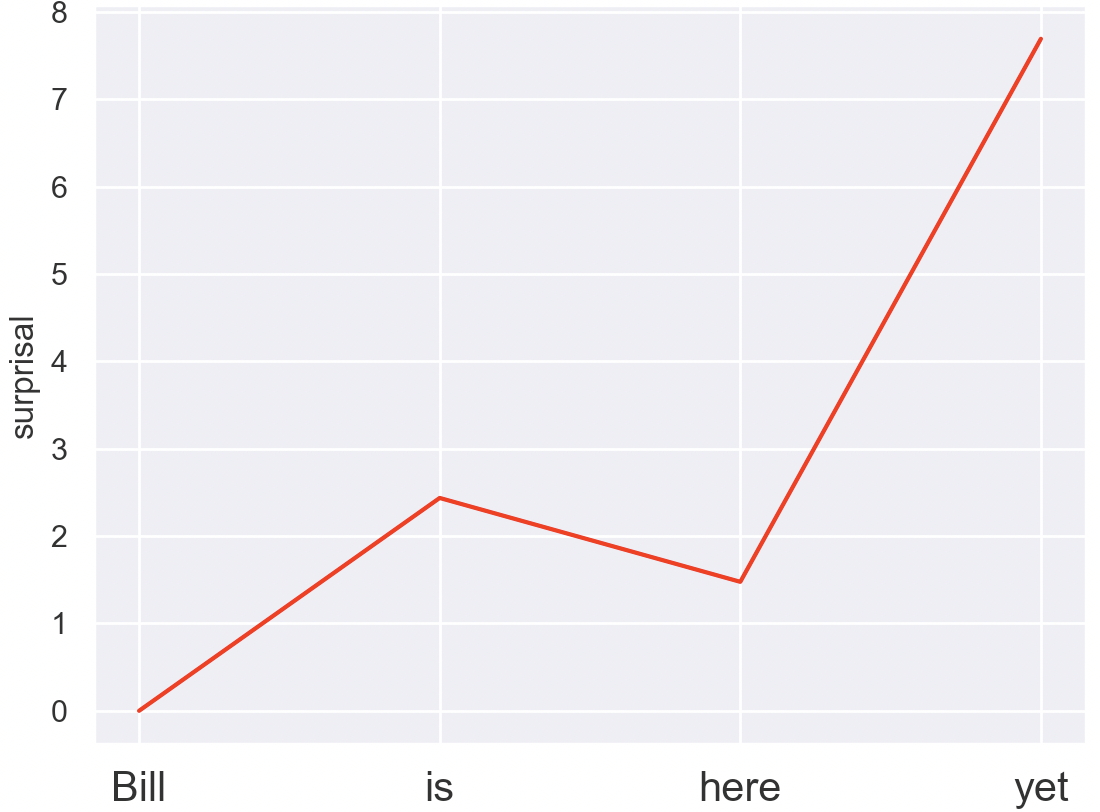
\includegraphics[width=.42\linewidth]{bad1} }}
    \qquad
    \subfloat[Grammatical]{{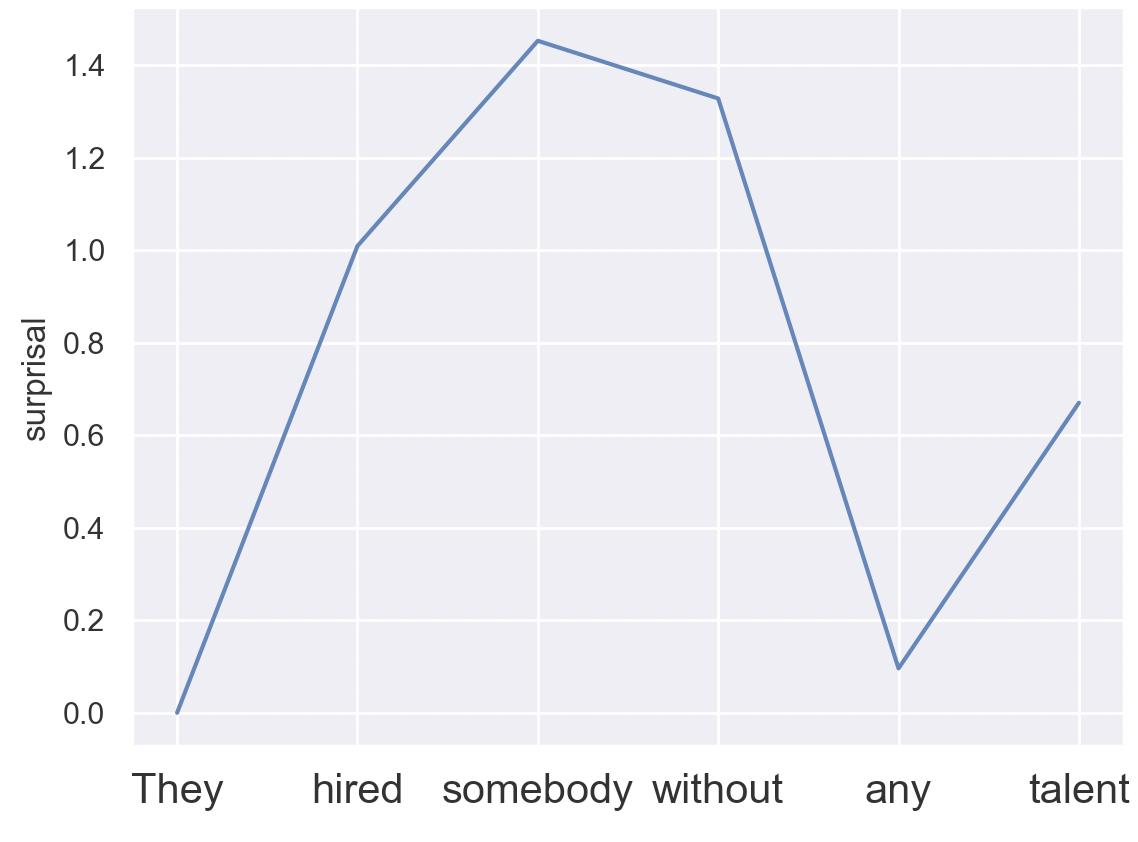
\includegraphics[width=.42\linewidth]{good2} }}
    \subfloat[Ungrammatical]{{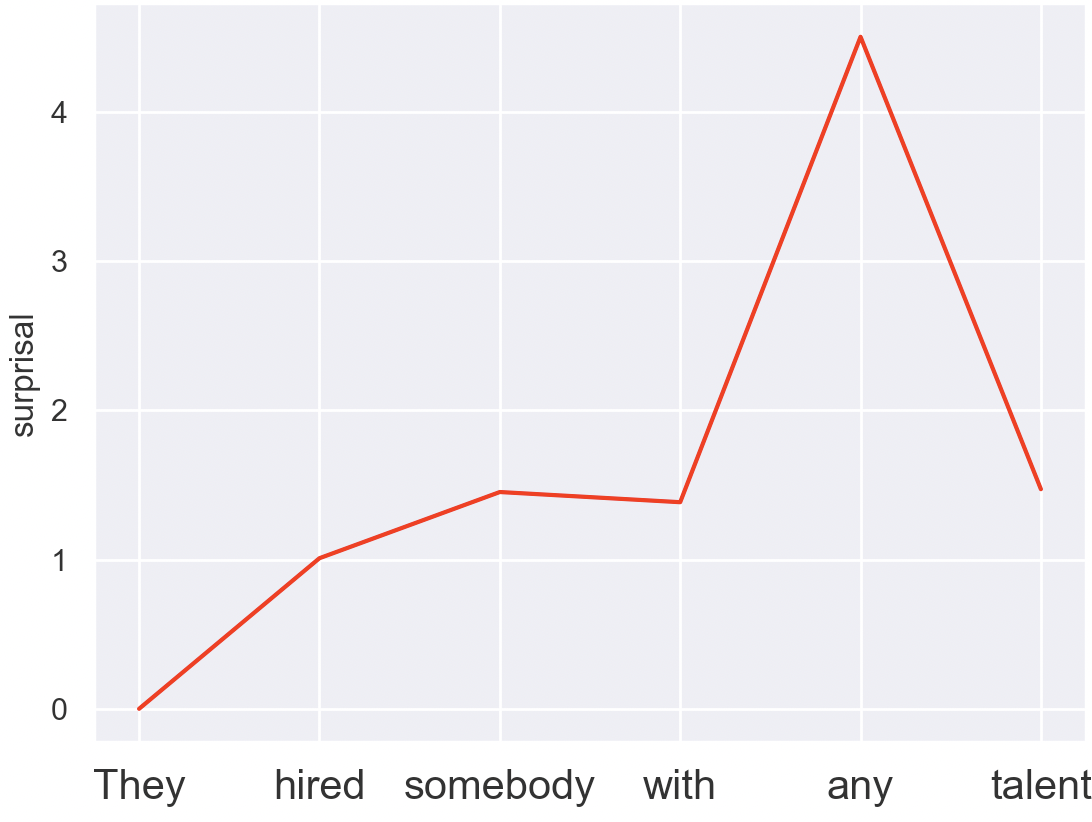
\includegraphics[width=.42\linewidth]{bad2} }}
    \caption{Plots of surprisal scores for words in the example sentences. Note that plots (a) and (c) are both contextually negative and plots (b) and (d) are positive. As expected, the surprisal score for the NPIs (\textit{yet} in plots (a) and (b) and \textit{any} in plots (c) and (d)) is much higher in positive contexts.}
    \label{fig:surprisal-basic-licensing}
\end{figure}

To determine the statistical significance of the surprisal scores of NPIs in different contexts, we computed surprisal scores for both variants of our 20 test items and computed the licensing interaction by taking pairwise differences. If the model had learned nothing at all about the NPI/licensor relation, we would expect the licensing interaction to be zero. However, if the model did learn to predict NPIs only in the presence of a licensor, then the licensing interaction should be positive. 

Measuring instantaneous surprisal upon encountering an NPI, we found a mean licensing interaction of 0.87, which we deemed significant ($t(19 = 1.82$, $p = 0.042$), so we reject the null hypothesis, concluding that the sentences containing a licensor had significantly lower suprisal than those without a licensor.

Measuring cumulative surprisal over the remainder of the clause, we found an even larger licensing interaction of 1.83, which we also deemed significant ($t(19) = 3.00$, $p = 0.004$).

Overall, this experiment shows that our LSTM model has at least a basic understanding of when negative polarity items should be expected.

\subsection{C-Command Relation Between Licensor and NPI}

As discussed in the the Introduction, there are structural restrictions on the NPI licensing relationship. For an NPI construction to be grammatical, it is not sufficient that a negative licensor precede the NPI in terms of linear word order. In fact, the licensor must c-command the NPI in order for the construction to be grammatical.

In the following example, the dependent clause is fixed as negative and the independent clause (which contains the NPI) is varied, so only the first variation is correct:
\begin{exe}
\ex
\begin{xlist}
\ex Because he was not tired, he was not even sleeping
\ex [*]{Because he was not tired, he was even sleeping} 
\end{xlist}
\end{exe}
In this subsection we attempt to determine whether LSTMs are capable of understanding syntactic structure with regards to negative polarity items. In order to do this we designed 10 base sentences. Each sentence begins with a negative clause, and the grammatically correct version has a second negative clause and NPI wheras the incorrect version has a second postive clause and NPI. We are motivated to analyze this type of interaction because a model that is well adjusted to NPI should determine that the presence of negative context in a separate c-command does not influence whether it is actually grammatical.

\subsection{Robustness of Negative Polarity Items to Intervening Material}
Syntactic dependencies are unchanged by the presence intervening material. In the following example, the presence of a negative polarity item (anymore) is due to syntactic licensing by negation (don't); modifying the object doesn't change the sentence structure, so it has no effect on NPI licensing:
\begin{exe}
\ex
\begin{xlist}
\ex We do not go to the supermarket anymore.
\ex We do not go to the supermarket that is owned by Mark anymore.
\ex We do not go down the block to the supermarket that is owned by Mark anymore. 
\end{xlist}
\end{exe}
We showed in the previous subsection that LSTMs have expectations for negative polarity items, so we attempt to determine whether those expectations remain over intervening material. For this subsection, we designed 10 sentences base sentences with NPI items. Each of the base sentences comes in three varieties: minimal intervening material (enough to make the sentence grammatical), 3-5 words of additional intervening material, and 6-10 additional words between the negative licensor and the polarity item. In all cases the intervening words modify the object of the base sentence.

\begin{figure*}
    \centering
    \subfloat[Base Sentence]{{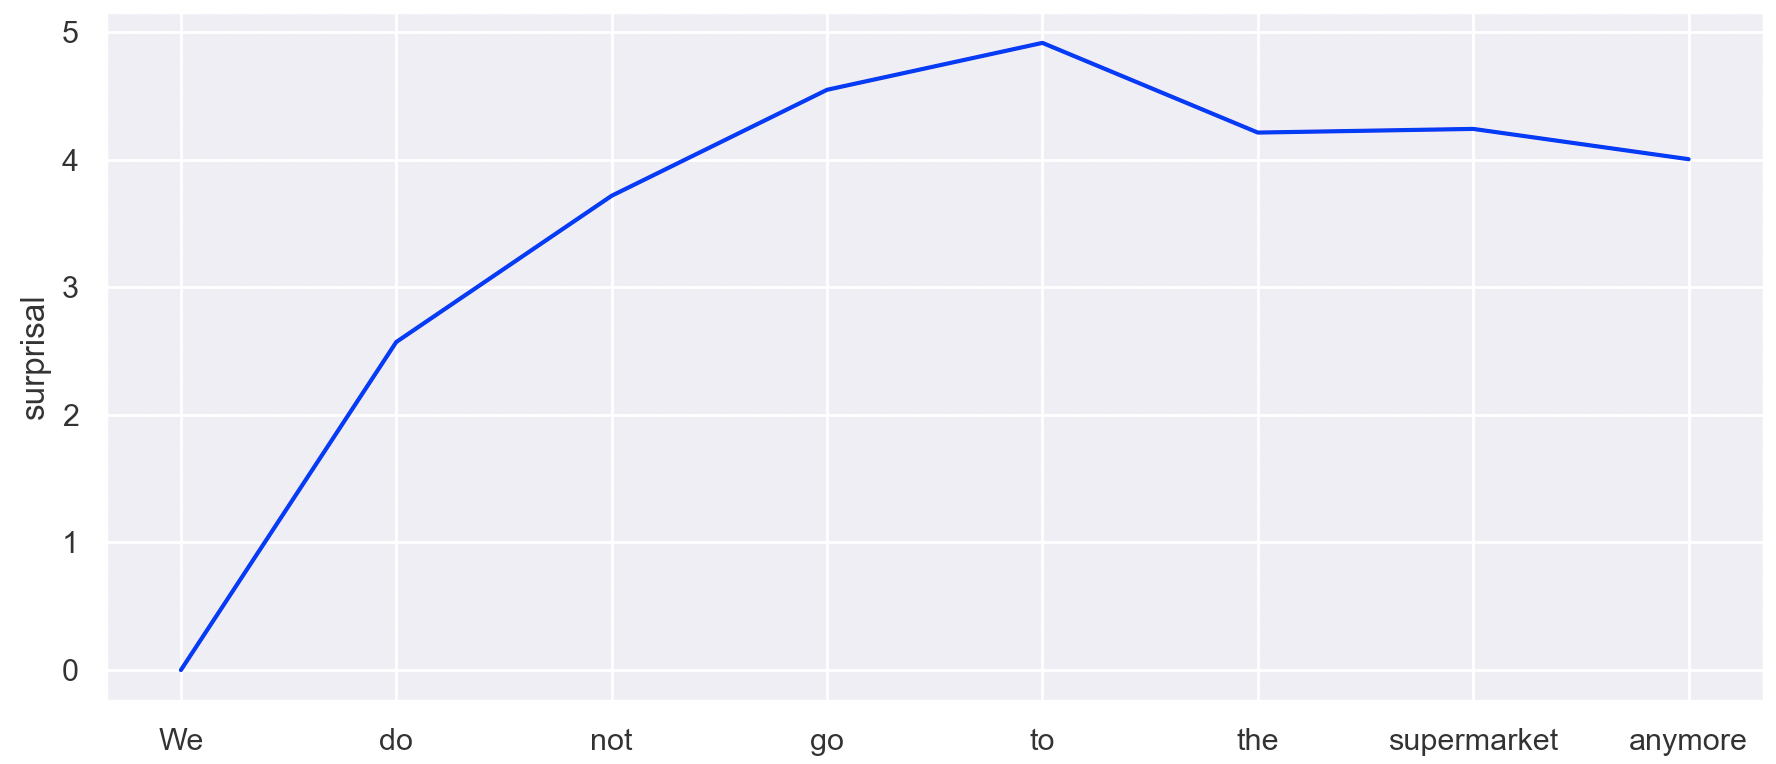
\includegraphics[width=.32\textwidth]{short} }}
    \subfloat[5 Additional Words]{{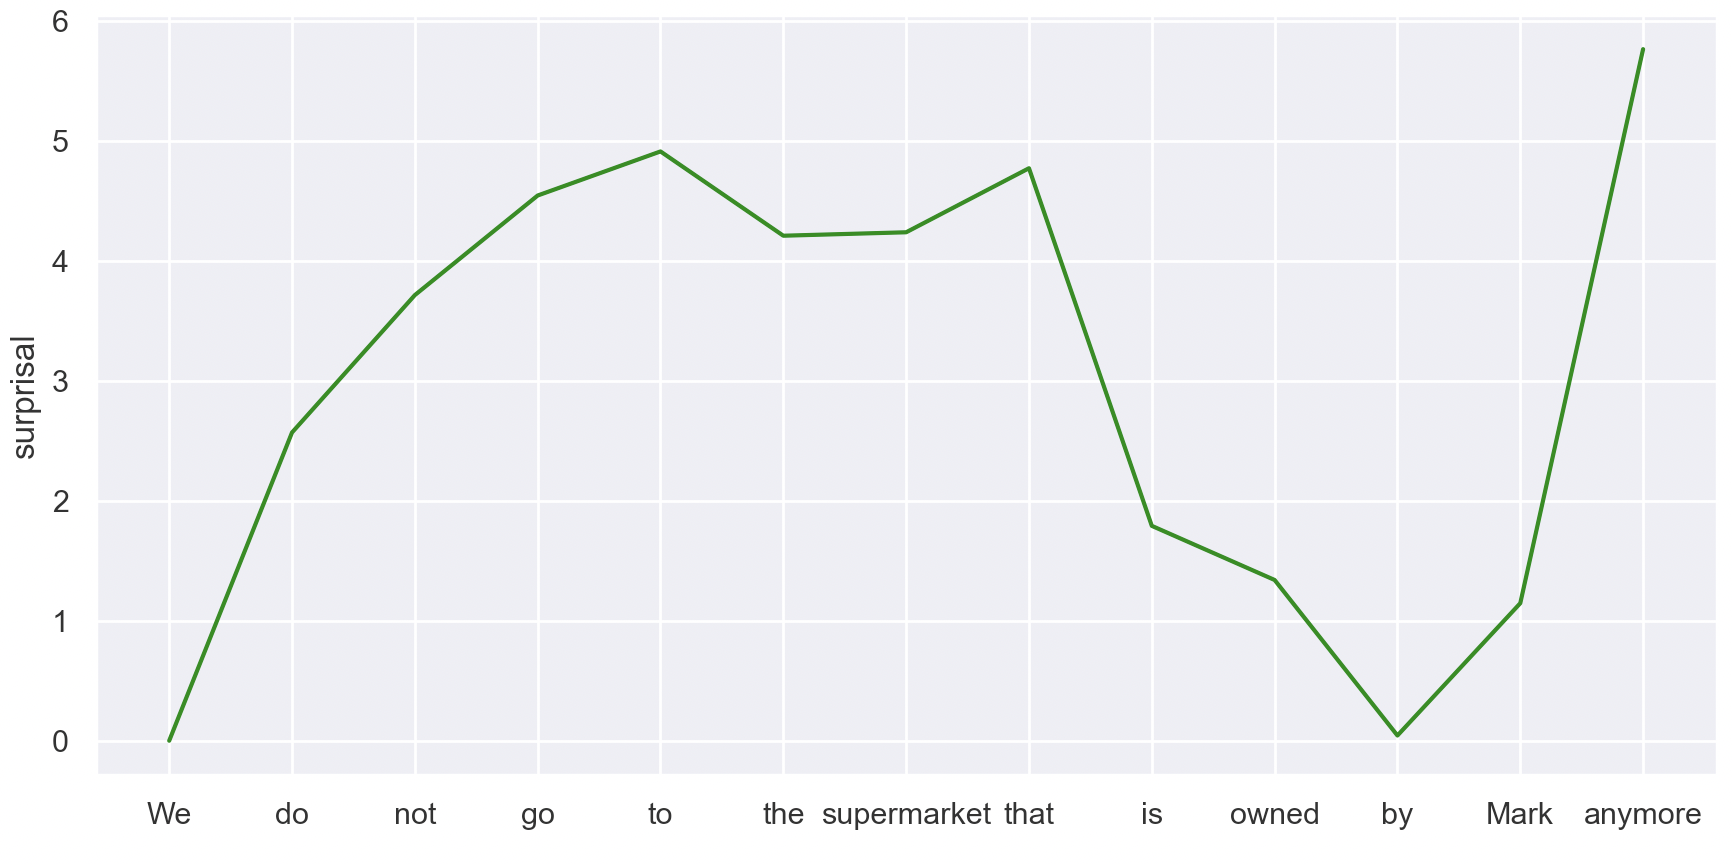
\includegraphics[width=.32\textwidth]{medium} }}
    \subfloat[8 Additional Words]{{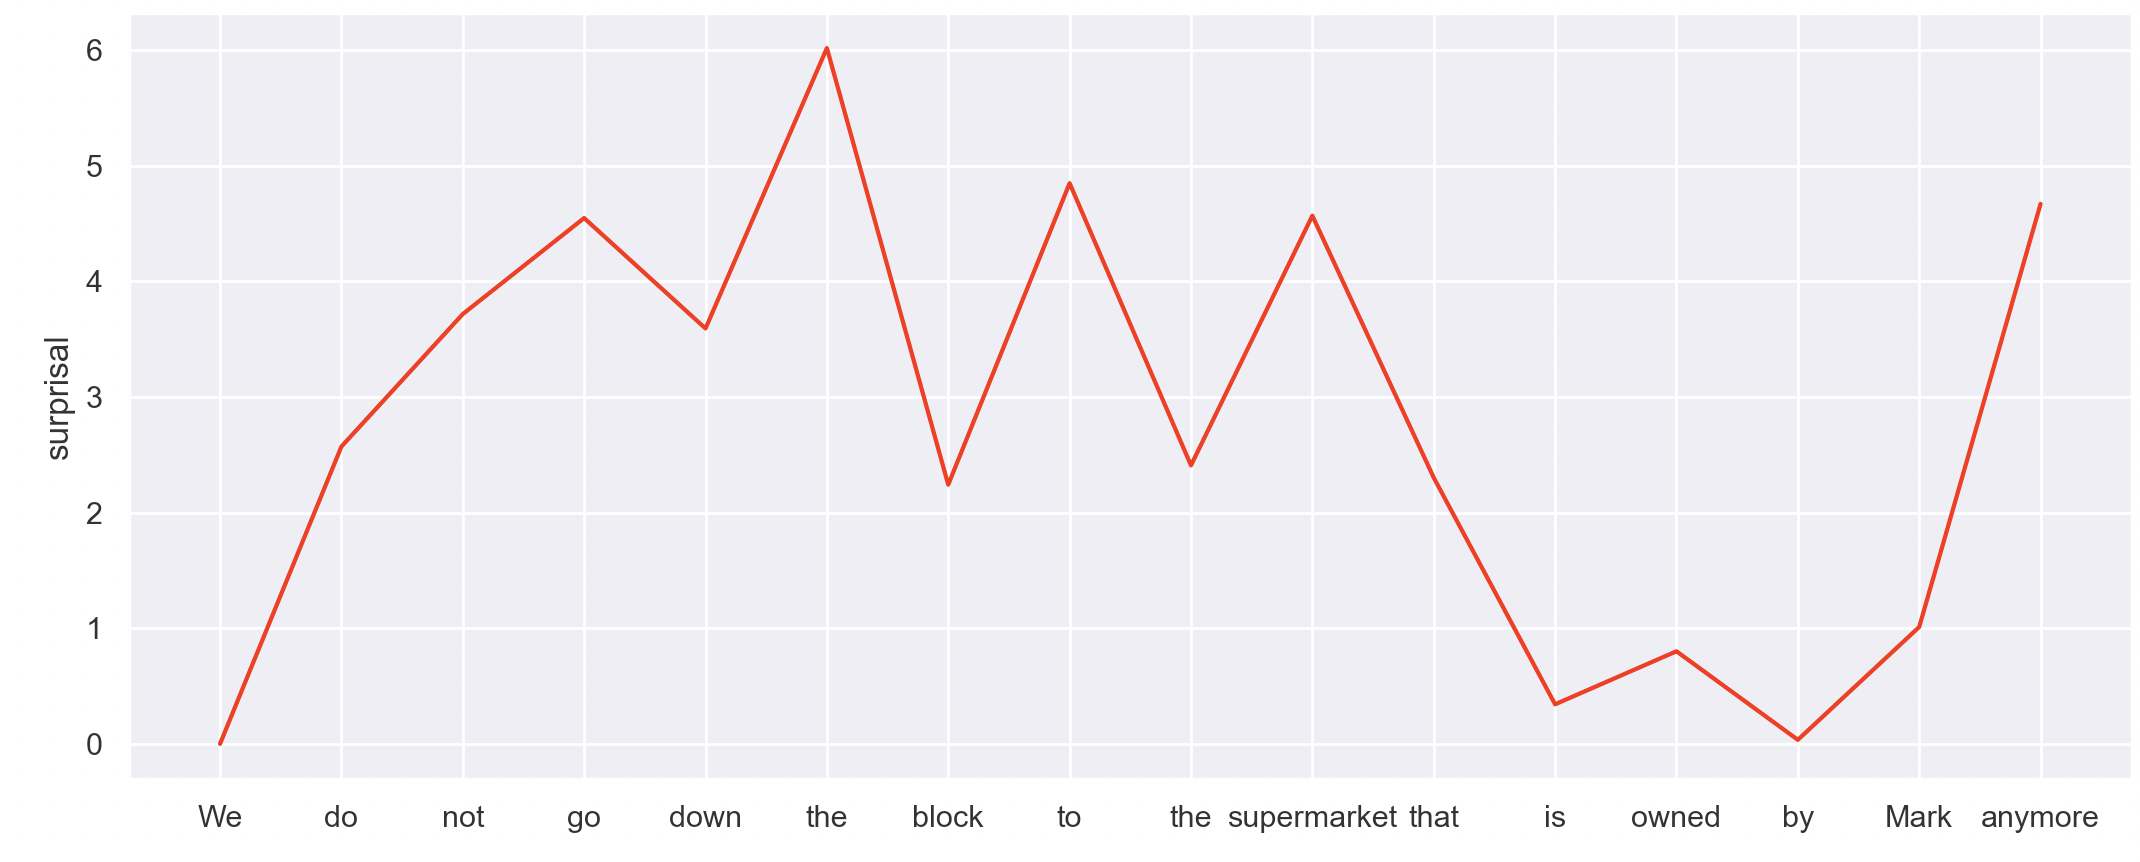
\includegraphics[width=.32\textwidth]{long} }}
    \caption{Plots of surprisal scores for words in the modified sentence. The surprisal score of the negative polarity item \textit{anymore} remains relatively unchanged by the amount of intervening material.}
\end{figure*}

An example of the results for this section are visualized in Figure 2. We found that in general, there was a weak positive correlation between the number of words in between the word that determined the negative context and the negative polarity item and the surprisal score. However as seen in the plots, the scores are relatively similar, so we can conclude that the model does not consider the NPIs as ungrammatical when the amount of intervening words is long.

\subsection{Ability to License Multiple Negative Polarity Items}
In most cases, a negative context can license multiple negative polarity items.
\begin{exe}
\ex
\begin{xlist}
\ex He didn't want to go with anybody anywhere
\ex [*]{He did want to go with anybody anywhere} 
\end{xlist}
\end{exe} 

\section{Results}

\bibliography{sources}

\end{document}
